%# -*- coding: utf-8 -*-
% tiling.tex
% asymptotebyexample 的一章,曲线绘制和编程入门

\chapter{André Deledicq 的铺砌插画}
\nocite{pstricks}

André 是一名兴趣广泛的法国数学教师,在他的新著《Le monde des pavages》(《铺
砌世界》)中,打算画一幅有关羊的铺砌插画:
\begin{figure}[H]
  \centering
  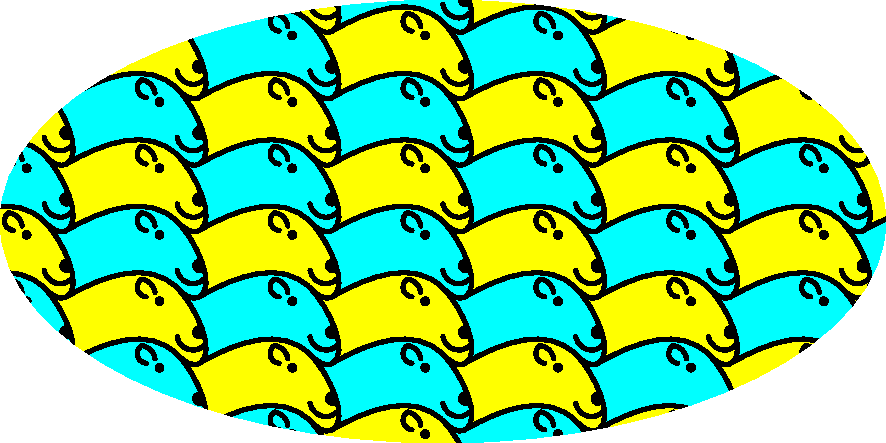
\includegraphics{tiling.pdf}
  \caption{André 理想中的铺砌图}
  \label{fig:tiling}
\end{figure}

André 很清楚他要画的图形的数学理论,但 André 的朋友 Timothy 告诉他要画这样
的图形多少是需要一些编程的知识的,对于他这样一位往日对计算机并不通晓的人来说
可能会有困难。不过 André 并不以为意:这世上还有什么比数学更难的呢?于是他兴
致勃勃的开始了。

\section{从矩形到铺砌}

铺砌图,顾名思义,就是像铺地板砖一样,把许多相同样式的图形平铺开来。不过,并
不是什么图形都可以平铺填满整个平面的——比如圆形就不行。把许多圆形一个挨一个
排列起来,也只能得到
\begin{figure}[H]
\centering
\begin{asy}
size(0,2cm);
for (int i = 0; i < 3; ++i)
    for (int j = 0; j < 10; ++j)
        filldraw(circle((j,i), 0.5), lightblue);
\end{asy}
\end{figure}
\noindent 或者是
\begin{figure}[H]
\centering
\begin{asy}
size(0,2cm);
for (int i = 0; i < 3; ++i)
    for (int j = 0; j < 10; ++j)
        filldraw(circle((j+0.5(i%2),sqrt(3)/2*i), 0.5), lightblue);
\end{asy}
\end{figure}
\noindent 都会留下许多空隙。而矩形、平行四边形、六边形等等都可以不留空隙地把平面铺满。

但问题是,如何设计出 André 理想中的那种看起来形状不规则的铺砌图案呢?

身为数学教师的 André 当然有办法。其实不规则铺砌图案还是规则图案的变形。
André 要画的羊形铺砌图,其实就是从矩形铺砌变化而来的。只要把一个矩形图案的上
下两边、左右两边分别变形,使得变形后的上边与下边、左边与右边还对应重合,就依
然可以完美地拼合起来。这正是铺砌图案最基本的构成方式:
\begin{figure}[H]
\centering
\begin{asy}
size(0,5cm);
defaultpen(linewidth(1mm));
path rec = box((0,0), (2,1));
draw(rec);

draw(shift(3,0)*rec, gray+0.5mm);
guide left = (0,1) -- (-0.2,0.8) -- (0,0.6) -- (0.1,0.1) -- (0,0);
guide bot = (0,0) -- (0.2,0.1) -- (1.6,-0.1) -- (2,0);
draw(shift(3,0) * (left ^^ shift(2,0)*left), heavyblue);
draw(shift(3,0) * (bot ^^ shift(0,1)*bot), heavygreen);

guide shape = left & bot & shift(2,0)*reverse(left)
    & shift(0,1)*reverse(bot) & cycle;
for (int i = 0 ; i < 2; ++i)
    for (int j = 0; j < 4; ++j)
	filldraw(shift(0.5+j,-1.5+0.5i)*scale(0.5)*shape, lightblue);
\end{asy}
\end{figure}

有了这个方法,对复杂的铺砌图,也只要从一个基本形状(比如矩形、正六边形)开始
变形,就等到铺砌所需要的一块“砖”。

因此,要画出羊头形状铺砌图,只要把一个矩形按照上面的要求变形为一个羊头形状,
在不同的位置重复画出就可以了。

\section{变量与曲线}

下面的问题就是,怎么画一个羊头呢?更具体地说,怎么画出羊头的曲线呢?

那么,首先要了解如何在 \Asy{} 中描述曲线。\ref{sec:linedraw} 节中提到 |--| 连
结一组坐标就成为直(折)线段;类似地,用 |..| 连结坐标就得到经过这些坐标点的
曲线:
\begin{lstlisting}
size(5cm,0);
pair z1 = (0,1), z2 = (1,1), z3 = (2,1),
     z4 = (0,0), z5 = (1,0), z6 = (2,0);
path p = z4 .. z1 .. z2 .. z6;
draw(p, gray+2mm);
\end{lstlisting}
\begin{figure}[H]
  \centering
\begin{asy}
settings.tex = "xelatex";
size(5cm,0);
pair z1 = (0,1), z2 = (1,1), z3 = (2,1),
     z4 = (0,0), z5 = (1,0), z6 = (2,0);
path p = z4 .. z1 .. z2 .. z6;
draw(p, gray+2mm);
dot(Label("1", align=NW), z1);
dot(Label("2", align=NE), z2);
dot("3", z3);
dot("4", z4);
dot("5", z5);
dot("6", z6);
\end{asy}
\end{figure}

在这里,我们定义了一些变量\index{变量}以使代码清晰(这里略去了画点和标签的代
码)。|pair|\index{pair@\lstinline=pair=} 类型的变量 |z1|, \ldots, |z6| 保存
六个坐标\index{坐标},|path|\index{path@\lstinline=path=} 类型的变量 |p| 保存
一条曲线路径\index{路径}。因而上面 |size| 之后的绘图代码就相当于
\begin{lstlisting}
draw( (0,0) .. (0,1) .. (1,1) .. (2,0), gray+2mm );
\end{lstlisting}
其中前面的一句 |size(5cm,0)|\index{size@\lstinline=size=} 表示代码中的坐标只
是相对位置,最后将整个图形按比例放缩为 $5$\,cm 宽\footnote{注意坐标、图形会被
放缩,但画笔的宽度不会放缩。}。类似地,也可以使用 |size(0,4cm)| 把图形放缩到
$4$\,cm 高。

最重要的当然还是曲线的表示。以 |..| 连结的坐标会以一种尽量接近圆弧的方式连为
经过这些点的光滑曲线。与画直线类似,|cycle|\index{cycle@\lstinline=cycle=} 可
以作为一个特殊的坐标产生闭合曲线,即一条闭路径\index{路径!闭路径}:
\begin{lstlisting}
path q = z4 .. z1 .. z2 .. z6 .. cycle;
draw(q, gray+2mm);
\end{lstlisting}
\begin{figure}[H]
  \centering
\begin{asy}
settings.tex = "xelatex";
size(5cm,0);
pair z1 = (0,1), z2 = (1,1), z3 = (2,1),
     z4 = (0,0), z5 = (1,0), z6 = (2,0);
path q = z4 .. z1 .. z2 .. z6 .. cycle;
draw(q, gray+2mm);
dot(Label("1", align=NW), z1);
dot(Label("2", align=NE), z2);
dot("3", z3);
dot("4", z4);
dot("5", z5);
dot("6", z6);
\end{asy}
\end{figure}

变量不仅仅是给了坐标、路径等对象一个简洁的名字,它也使得对同一个对象重复使用
并进行不同的操作变得十分方便:
\begin{lstlisting}
fill(q, lightblue);
draw(q, gray+2mm);
\end{lstlisting}
\begin{figure}[H]
  \centering
\begin{asy}
settings.tex = "xelatex";
size(5cm,0);
pair z1 = (0,1), z2 = (1,1), z3 = (2,1),
     z4 = (0,0), z5 = (1,0), z6 = (2,0);
path q = z4 .. z1 .. z2 .. z6 .. cycle;
fill(q, lightblue);
draw(q, gray+2mm);
dot(Label("1", align=NW), z1);
dot(Label("2", align=NE), z2);
dot("3", z3);
dot("4", z4);
dot("5", z5);
dot("6", z6);
\end{asy}
\end{figure}

\endinput

% vim:tw=77:

